\setcounter{page}{1}
\section*{Zielsetzung}
Im Versuch 61 sollen die Grundlagen der Lasertechnik kennengelernt werden. Hierzu werden zunächst die
wichtigsten theoretischen Grundlagen erarbeitet und anschließend die Eigenschaften eines Helium-Neon-Lasers
experimentell untersucht.
\section{Theorie}
Laser sind optische Geräte, mit denen möglichst monochromatisches Licht hoher Kohärenz, Intensität und gegebenenfalls
Polarisation erzeugt werden soll.
Anhand der Quellen \cite{anleitung61} und \cite{dem} wird im Folgenden die theoretische Funktionsweise eines Lasers
erläutert. Zur Untersuchung der Wechselwirkung eines Strahlungsfeldes mit einem System aus Atomen bzw. Molekülen
wird das theoretische Modell eines Zweiniveausystems verwendet.
\subsection{Zweiniveausystem}
Als vereinfachtes Modell soll ein System mit den Zuständen $\ket{1}$ und $\ket{2}$ und zugehörigen Energieeigenwerten
$E\ua{1}$ und $E\ua{2}$ (mit $E\ua{2}> E\ua{1}$) betrachtet werden. Ein externes Strahlungsfeld sei durch die spektrale Energiedichte $\rho(\nu)$
charakterisiert. Durch die induzierte Absorption eine Photons der Energie $h \nu = E\ua{2} - E\ua{1}$ kann das
System in den Zustand $\ket{2}$ angeregt werden. Die Wahrscheinlichkeit $P\ua{1\rightarrow 2}$ für diesen Prozess ist proportional
zur spektrale Energiedichte $\rho(\nu)$
\begin{equation}
  P\ua{1\rightarrow 2} = B\ua{1\rightarrow 2}\cdot\rho(\nu).
\end{equation}
Der Proportionalitätsfaktor $B\ua{1\rightarrow 2}$ wird als Einsteinkoeffizient der induzierten Absorption bezeichnet. Analog kann
eine induzierte Emission stattfinden mit der Wahrscheinlichkeit
\begin{equation}
  P\ua{2\rightarrow 1} = B\ua{2\rightarrow 1}\cdot\rho(\nu).
\end{equation}
Mit dem Einsteinkoeffizienten der induzierten Emission $B\ua{2\rightarrow1}$.
Das induzierte Photon stimmt in Energie, Phase und Ausbreitungsrichtung mit dem anregenden Photon überein.
Unabhängig vom externen Strahlungsfeld
kann auch spontan ein Photon emittiert werden
\begin{equation}
  P\ua{s} = A\ua{2 \rightarrow 1}.
\end{equation}
Mit dem Einsteinkoeffizienten der spontanen Emission $A\ua{2 \rightarrow 1}$. Im thermischen Gleichgewicht folgen die Besetzungszahlen
$n\ua{i}$ der Niveaus einer Boltzmann-Statistik
\begin{equation}
  n\ua{i} = \frac{g\ua{i}n}{Z}\exp\left\{-\frac{E\ua{i}}{k\ua{B}T}\right\}.
\end{equation}
Hierbei ist $n$ die Gesamtzahl der Systeme, $g\ua{i}$ das statistische Gewicht des Zustands $\ket{i}$ und $Z$ die Zustandssumme. Im thermischen
Gleichgewicht dominiert somit die Besetzung des Grundzustandes. Die Aufgabe eines Lasers besteht nun darin,
eine dauerhafte Verstärkung des Strahlungsfeldes zu erzeugen.
\subsection{Funktionsprinzip eines Lasers}
Ein Laser besteht prinzipiell aus einem aktiven Lasermedium, einer Pumpquelle und einem Resonator. Die Pumpquelle sorgt dafür, dass
mindestens ein angeregter Zustand im Medium häufiger auftritt als ein darunter liegender. Diese Situation wird als Besetzungsinversion bezeichnet. Als direkte
Folge sollen im Medium mehr induzierte Emissionen als spontane Emissionen stattfinden, was dazu führt, dass das Strahlungsfeld durch das Medium verstärkt wird.
Der Resonator bewirkt, dass der Laufweg der Photonen im Medium verlängert wird. Das Prinzip ist in Abbildung \ref{fig: prinzip_laser} dargestellt.
\begin{figure}
  \centering
  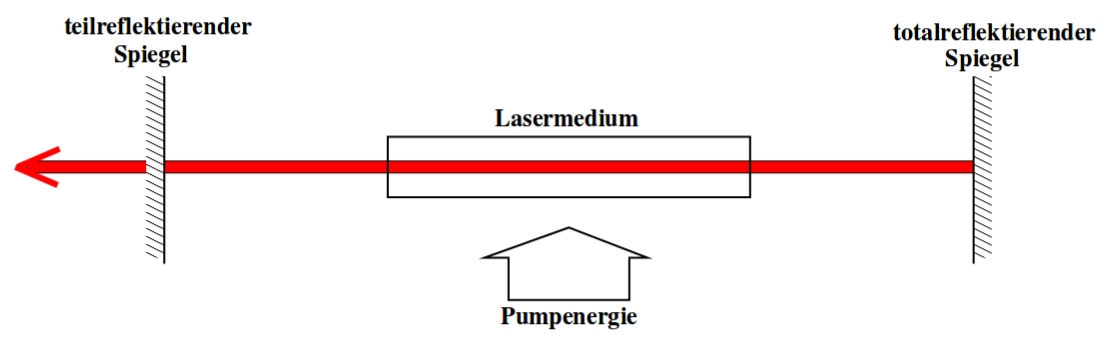
\includegraphics[width = 0.7\textwidth]{theorie_bilder/prinzip_laser.png}
  \caption{Darstellung der grundlegenden Komponenten eines Lasers \cite{anleitung61}.} %Finde Funktionsweise passt nicht so, er ist ja der Aufbau des Resonatros zu erkennen
  \label{fig: prinzip_laser}
\end{figure}

Optische Resonatoren sind durch gegenüberliegende Spiegel realisiert, von denen mindestens einer halbdurchlässig ist, um den erzeugten Strahl
auszukoppeln. Verluste an den offenen Rändern der Anordung werden inbesondere durch konfokale Anordnungen minimiert.
In Analogie zum mechanischen Problem eines eingespannten Seiles können nur solche Wellenlängen $\lambda$
im Resonator verstärkt werden, die
folgender Bedingung genügen
\begin{equation}
  \lambda = \frac{2 L }{n} \quad n \in  \mathbb{N}.
  \label{eq: longmoden}
\end{equation}
Mit dem Abstand der Spiegel $L$. Man spricht im Zusammenhang mit Lasern von longitudinalen Moden, die durch den Index $n$ bestimmt sind.
Durch die Bedingung \eqref{eq: longmoden} tritt eine Selektion der möglichen Wellenlängen auf. Innerhalb
einer natürlichen spektralen Verteilung, die insbesondere durch den optischen Dopplereffekt hervorgerufen wird, werden nur solche Wellenlängen
verstärkt, die die longitudinale Modenbedingung erfüllen.

Durch Beugungseffekte an Unebenheiten der Spiegel tritt eine Feldverteilung senkrecht zur Resonatorachse auf. Stationäre Intensitätsverteilungen
werden als transversale oder TEM-Moden (\textit{transverse electromagnetic}) bezeichnet. Die TEM Moden stehen in direkter Analogie zu den Eigenmoden
einer schwingenden eingespannten Membran (Trommel). Die Intensität $I\ua{00}$ der Grund- oder Fundamentalmode $T\ua{00}$ folgt einer Gaußverteilung
\begin{equation}
  I\ua{00}(d) = I\ua{0}\exp\left\{- 2\left(\frac{d-d_0}{w}\right)^2\right\}
  \label{eq: tem00}
\end{equation}
mit den freien Parametern $I\ua{0}$, $d_0$ und $w$ sowie dem senkrechten Abstand zur Resonatorachse $d$. Der Parameter $w$ wird auch als Radius
der Fundamentalmode bezeichnet. Die Mode $T\ua{01}$ kann durch folgende Funktion beschrieben werden
\begin{equation} % Ich würde anmerken, dass die T_01 Mode eigentlich symetrisch ist, und nur wegen der Messung asymetrisch ist.
  I\ua{01}(d) = I\ua{0, 1}\exp\left\{- 2\left(\frac{d-d_{0, 1}}{w_{1}}\right)^2\right\} + I\ua{0, 2}\exp\left\{- 2\left(\frac{d-d_{0,2}}{w_{2}}\right)^2\right\}.
  \label{eq: tem01}
\end{equation}
Dabei wird eine Asymmetrie in der Höhe der beiden Maxima zugelassen (i.A. $I\ua{0, 1} \neq I\ua{0, 2}$), die theoretisch nicht
erwartet wird.

Allgemein stellt sich eine stabile Modenverteilung
ein, wenn die folgende Stabilitätbedingung erfüllt ist
\begin{equation}
  0 \leq g_1 g_2 \leq 1.
  \label{eq: stabilität}
\end{equation}
Wobei
\begin{equation}
  g\ua{i} = 1 - L/r\ua{i}
  \label{eq: spiegelparameter}
\end{equation}
mit dem jeweiligen Krümmungsradius $r\ua{i}$ der Spiegel. Das Produkt $g_1g_2$
als Funktion des Spiegelsabstandes $L$ ist für $r\ua{2} = \SI{1400}{\meter}$ in Abbildung~\ref{fig: stabilitätsbedingung} dargestellt.
Für einen ebenen Spiegel ("$r_1 = \infty$") ist die Bedingung \eqref{eq: stabilität} erfüllt für
\begin{equation}
  \SI{0}{\meter}\leq L \leq \SI{1.4}{\meter}.
\end{equation}
Bzw. für $r_1 = \SI{1400}{\milli\meter}$
\begin{equation}
  \SI{0}{\meter} \leq L \leq \SI{2.8}{\meter}.
\end{equation}
\begin{figure}
  \centering
  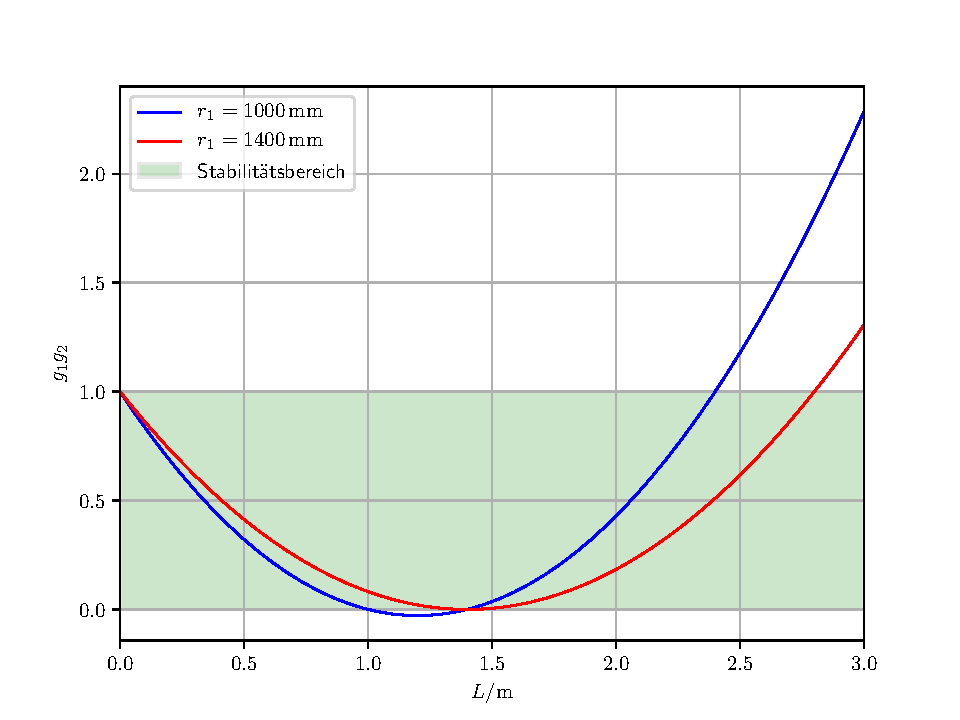
\includegraphics[width = \textwidth]{theorie_bilder/g_1_g_2.pdf}
  \caption{Darstsellung der Stabilitätsbedingung \eqref{eq: stabilität}. Hierbei gilt jeweils \\$r_2 = \SI{1400}{\milli\meter}$.}
  \label{fig: stabilitätsbedingung}
\end{figure}

\subsection{\ce{HeNe}-Laser }
Als Resonatormedium wird beim \ce{HeNe}-Laser ein Gemisch aus einem Teil Helium und fünf Teilen Neon verwendet, das unter einem Druck von
ca. $\SI{1}{\milli\bar}$ in einem Glaskolben isoliert ist. Das eigentliche Lasermedium ist Neon, während Helium zum Pumpen verwendet wird.
Die Erzeugung der notwendigen Besetzungsinversion ist in Abbildung~\ref{fig: energieschema} dargestellt. Durch eine Gasentladung werden
die Heliumatome angeregt, welche wiederum durch Stöße zweiter Art die Neon Atome anregen können. Hierbei sind vorallem die sehr stabilen Zustände
$2^1s$ und $2^3s$ des Helium verantwortlich, deren Anregungsenergie im Rahmen einer natürlichen Linienbreite die in \ref{fig: energieschema}
eingezeichneten Neon Zustände anregen können. Da die mittlere Lebensdauer des $5s$ Zustandes größer ist als jene des $3p$ Zustandes, tritt die gewünschte
Asymmetrie in den Besetzungszahlen zweier Energienieveaus auf. Stimulierte Emissionsprozesse vom $5s$ in den $3p$ Zustand sind durch die Langlebigkeit
des $5s$-Niveaus pro Zeiteinheit wahrscheinlicher als spontane Emission\footnote{Das eingangs beschriebene Zwei-Niveau-System kann eine solche
Asymmetrie nicht erzeugen, da induzierte Absorptionen und Emissionen in gleichem Maße auftreten würden.}.
Die betreffende Spektrallinie des Übergangs zwischen den beiden Neon Niveaus liegt mit $\lambda = \SI{632.8}{\nano\meter}$ im sichtbaren
roten Bereich des elektromagnetischen Spektrums.
\begin{figure}
  \centering
  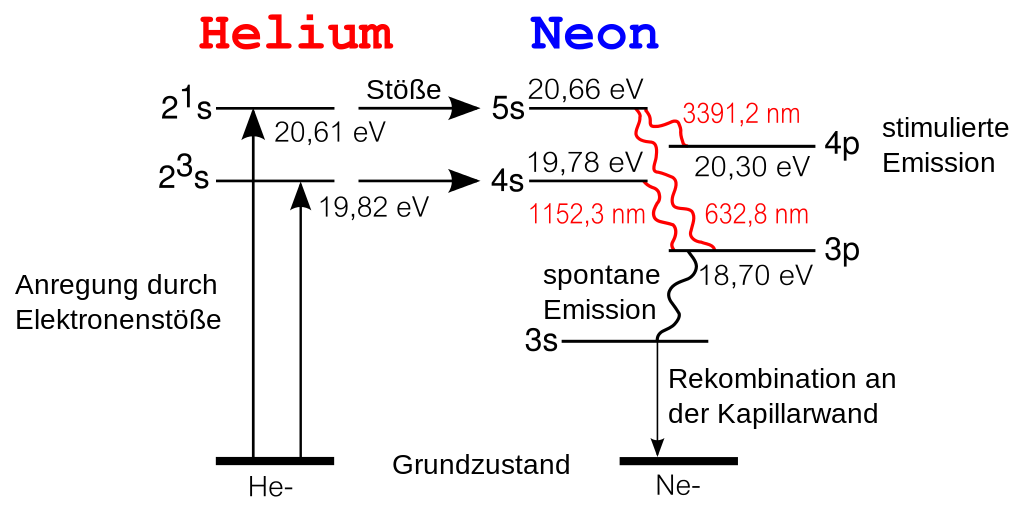
\includegraphics[width = 0.8\textwidth]{theorie_bilder/energieschema.png}
  \caption{Darstellung des für den \ce{HeNe}-Laser relevanten Energieschemas \cite{wiki}.}
  \label{fig: energieschema}
\end{figure}
